% Options for packages loaded elsewhere
\PassOptionsToPackage{unicode}{hyperref}
\PassOptionsToPackage{hyphens}{url}
%
\documentclass[
  ignorenonframetext,
  aspectratio=169,
]{beamer}
\usepackage{pgfpages}
\setbeamertemplate{caption}[numbered]
\setbeamertemplate{caption label separator}{: }
\setbeamercolor{caption name}{fg=normal text.fg}
\beamertemplatenavigationsymbolsempty
% Prevent slide breaks in the middle of a paragraph
\widowpenalties 1 10000
\raggedbottom
\setbeamertemplate{part page}{
  \centering
  \begin{beamercolorbox}[sep=16pt,center]{part title}
    \usebeamerfont{part title}\insertpart\par
  \end{beamercolorbox}
}
\setbeamertemplate{section page}{
  \centering
  \begin{beamercolorbox}[sep=12pt,center]{part title}
    \usebeamerfont{section title}\insertsection\par
  \end{beamercolorbox}
}
\setbeamertemplate{subsection page}{
  \centering
  \begin{beamercolorbox}[sep=8pt,center]{part title}
    \usebeamerfont{subsection title}\insertsubsection\par
  \end{beamercolorbox}
}
\AtBeginPart{
  \frame{\partpage}
}
\AtBeginSection{
  \ifbibliography
  \else
    \frame{\sectionpage}
  \fi
}
\AtBeginSubsection{
  \frame{\subsectionpage}
}

\usepackage{amsmath,amssymb}
\usepackage{iftex}
\ifPDFTeX
  \usepackage[T1]{fontenc}
  \usepackage[utf8]{inputenc}
  \usepackage{textcomp} % provide euro and other symbols
\else % if luatex or xetex
  \usepackage{unicode-math}
  \defaultfontfeatures{Scale=MatchLowercase}
  \defaultfontfeatures[\rmfamily]{Ligatures=TeX,Scale=1}
\fi
\usepackage{lmodern}
\usecolortheme{whale}
\ifPDFTeX\else  
    % xetex/luatex font selection
\fi
% Use upquote if available, for straight quotes in verbatim environments
\IfFileExists{upquote.sty}{\usepackage{upquote}}{}
\IfFileExists{microtype.sty}{% use microtype if available
  \usepackage[]{microtype}
  \UseMicrotypeSet[protrusion]{basicmath} % disable protrusion for tt fonts
}{}
\makeatletter
\@ifundefined{KOMAClassName}{% if non-KOMA class
  \IfFileExists{parskip.sty}{%
    \usepackage{parskip}
  }{% else
    \setlength{\parindent}{0pt}
    \setlength{\parskip}{6pt plus 2pt minus 1pt}}
}{% if KOMA class
  \KOMAoptions{parskip=half}}
\makeatother
\usepackage{xcolor}
\newif\ifbibliography
\setlength{\emergencystretch}{3em} % prevent overfull lines
\setcounter{secnumdepth}{-\maxdimen} % remove section numbering


\providecommand{\tightlist}{%
  \setlength{\itemsep}{0pt}\setlength{\parskip}{0pt}}\usepackage{longtable,booktabs,array}
\usepackage{calc} % for calculating minipage widths
\usepackage{caption}
% Make caption package work with longtable
\makeatletter
\def\fnum@table{\tablename~\thetable}
\makeatother
\usepackage{graphicx}
\makeatletter
\def\maxwidth{\ifdim\Gin@nat@width>\linewidth\linewidth\else\Gin@nat@width\fi}
\def\maxheight{\ifdim\Gin@nat@height>\textheight\textheight\else\Gin@nat@height\fi}
\makeatother
% Scale images if necessary, so that they will not overflow the page
% margins by default, and it is still possible to overwrite the defaults
% using explicit options in \includegraphics[width, height, ...]{}
\setkeys{Gin}{width=\maxwidth,height=\maxheight,keepaspectratio}
% Set default figure placement to htbp
\makeatletter
\def\fps@figure{htbp}
\makeatother

%% Set numering of slides
\setbeamertemplate{navigation symbols}{} 
\setbeamertemplate{footline}[page number]
\titlegraphic{
  
\includegraphics[width=2cm]{style/UZH.jpg}
  \hspace*{2cm}~%
  
\includegraphics[width=2cm]{style/FHNW.png}
  \hspace*{2cm}~%
  
\includegraphics[width=1cm]{style/BFH.png}
  }
\makeatletter
\@ifpackageloaded{caption}{}{\usepackage{caption}}
\AtBeginDocument{%
\ifdefined\contentsname
  \renewcommand*\contentsname{Table of contents}
\else
  \newcommand\contentsname{Table of contents}
\fi
\ifdefined\listfigurename
  \renewcommand*\listfigurename{List of Figures}
\else
  \newcommand\listfigurename{List of Figures}
\fi
\ifdefined\listtablename
  \renewcommand*\listtablename{List of Tables}
\else
  \newcommand\listtablename{List of Tables}
\fi
\ifdefined\figurename
  \renewcommand*\figurename{Figure}
\else
  \newcommand\figurename{Figure}
\fi
\ifdefined\tablename
  \renewcommand*\tablename{Table}
\else
  \newcommand\tablename{Table}
\fi
}
\@ifpackageloaded{float}{}{\usepackage{float}}
\floatstyle{ruled}
\@ifundefined{c@chapter}{\newfloat{codelisting}{h}{lop}}{\newfloat{codelisting}{h}{lop}[chapter]}
\floatname{codelisting}{Listing}
\newcommand*\listoflistings{\listof{codelisting}{List of Listings}}
\makeatother
\makeatletter
\makeatother
\makeatletter
\@ifpackageloaded{caption}{}{\usepackage{caption}}
\@ifpackageloaded{subcaption}{}{\usepackage{subcaption}}
\makeatother
\ifLuaTeX
  \usepackage{selnolig}  % disable illegal ligatures
\fi
\usepackage{bookmark}

\IfFileExists{xurl.sty}{\usepackage{xurl}}{} % add URL line breaks if available
\urlstyle{same} % disable monospaced font for URLs
\hypersetup{
  pdftitle={Data Anonymization for Open Science},
  pdfauthor={Jiří Novák; Marko Miletić; Oscar Thees; Alžběta Beranová},
  hidelinks,
  pdfcreator={LaTeX via pandoc}}

\title{Data Anonymization for Open Science}
\subtitle{useR! 2024}
\author{Jiří Novák\inst{1,2} \and Marko Miletić\inst{3} \and Oscar
Thees\inst{2} \and Alžběta Beranová\inst{4}}
\date{July 8, 2024}
\institute{\inst{1} University of Zurich \inst{2} University of Applied
Sciences Northwestern Switzerland \and \inst{3} Bern University of
Applied Sciences \inst{4} Czech Statistical Office}

\begin{document}
\frame{\titlepage}

\begin{frame}
\vspace{12em}

Jiří Novák CC BY-NC-ND (2024)


\includegraphics{style/by-nc-nd.png}

This license enables reusers to copy and distribute the material in any
medium or format in unadapted form only, for noncommercial purposes
only, and only so long as attribution is given to the creator.
\end{frame}

\begin{frame}{About Speakers}
\phantomsection\label{about-speakers}
\textbf{Jiří Novák}

\begin{itemize}
\tightlist
\item
  Ph.D.~in Statistics with topic Simulation of Synthetic Microdata
\item
  Statistical confidentiality of Czech Census 2021
\end{itemize}

\pause

\textbf{Marko Miletić}

\begin{itemize}
\item
  \color{red}{XXX}
\item
  \color{red}{XXX}
\end{itemize}

\pause

\textbf{Oscar Thees}

\begin{itemize}
\item
  \color{red}{XXX}
\item
  \color{red}{XXX}
\end{itemize}

\pause

\textbf{Alžběta Beranová}

\begin{itemize}
\item
  \color{red}{XXX}
\end{itemize}
\end{frame}

\begin{frame}{Data Anonymization in which context?}
\phantomsection\label{data-anonymization-in-which-context}
This tutorial is about Data Anonymization in the context of the field of
Statistical Disclosure Control (SDC).

SDC is also known as Statistical disclosure limitation or Disclosure
avoidance.

\vspace{1cm}

\textbf{Statistical Disclosure Control} seeks to protect statistical
data in such a way that they can be released without giving away
confidential information that can be linked to specific individuals or
entities.
\end{frame}

\begin{frame}{Importance of Data Anonymization}
\phantomsection\label{importance-of-data-anonymization}
There are several main reasons:

\begin{enumerate}
\item
  \textbf{Principle} It is a fundamental principle of Official
  Statistics that the statistical records of individual persons,
  businesses, or events used to produce Official Statistics are strictly
  confidential and to be used only for statistical purposes.
\item
  \textbf{Legal} Legislation imposes a legal obligation to protect
  individual business and personal data. Legal frameworks regulate what
  is allowed and what is not allowed regarding the publication of
  private information.
\item
  \textbf{Quality} Respondents need confidence in the preservation of
  the confidentiality of individual information. If they do not trust
  the confidentiality of the data, they may not provide accurate
  information.
\item
  \textbf{Ethical} Disclosing information that can be linked to specific
  individuals or entities is unethical.
\end{enumerate}
\end{frame}

\begin{frame}{Relevance to Open Science}
\phantomsection\label{relevance-to-open-science}
\textbf{Open Science}, \textbf{Open Access}, \textbf{Open Data} are
important trends in the scientific community.

Research data that results from publicly funded research should be
\textbf{FAIR}: \newline \textbf{findable}, \textbf{accessible},
\textbf{interoperable}, \textbf{reusable}

\begin{itemize}
\item
  therefore replicable, transparent, trustworthy
\item
  Principle: as open as possible, as closed as necessary
\item
  Enables data sharing and collaboration
\item
  Facilitates reproducible research
\item
  Balances transparency with privacy
\end{itemize}

\href{https://eur-lex.europa.eu/eli/reco/2018/790/oj}{\color{blue}\underline{Commission Recommendation (EU) 2018/790 on access to and preservation}}
\href{https://eur-lex.europa.eu/eli/reco/2018/790/oj}{\color{blue}\underline{of scientific information}}
\end{frame}

\begin{frame}{Outputs to protect}
\phantomsection\label{outputs-to-protect}
Different outputs require different approaches to SDC and different
mixtures of tools.

\begin{itemize}
\tightlist
\item
  Macrodata (Tabular data)
\item
  Microdata
\item
  Dynamic databases
\item
  Statistical analyses
\end{itemize}

\vspace{1cm}

\textbf{Disclaimer}: Imposing a single solution for all types of data is
not possible. \newline This tutorial will focus on Microdata and Tabular
data.
\end{frame}

\begin{frame}{Key Concepts}
\phantomsection\label{key-concepts}
Key Concepts are:

\begin{itemize}
\tightlist
\item
  \textbf{Disclosure}

  \begin{itemize}
  \tightlist
  \item
    A disclosure occurs when a person or an organisation recognises or
    learns somethingthat they did not know already about another person
    or organisation, via released data.
  \end{itemize}
\end{itemize}

\pause

\begin{itemize}
\tightlist
\item
  \textbf{Re-identification risk}

  \begin{itemize}
  \tightlist
  \item
    Re-identification risk is the risk that an intruder can link a
    record in the released data to a specific individual in the
    population.
  \end{itemize}
\end{itemize}

\pause

\begin{itemize}
\tightlist
\item
  \textbf{Data utility}

  \begin{itemize}
  \tightlist
  \item
    Data utility is the usefulness of the data for the intended purpose.
  \end{itemize}
\end{itemize}
\end{frame}

\begin{frame}{Disclosure}
\phantomsection\label{disclosure}
A disclosure occurs when a person or an organisation recognises or
learns something that they did not know already about another person or
organisation, via released data.

Types of disclosure risk:

\begin{enumerate}
[(1)]
\tightlist
\item
  \textbf{Identity disclosure}
\item
  \textbf{Attribute disclosure}
\item
  \textbf{Inferential disclosure}
\end{enumerate}
\end{frame}

\begin{frame}{Disclosure}
\phantomsection\label{disclosure-1}
A disclosure occurs when a person or an organisation recognises or
learns something that they did not know already about another person or
organisation, via released data.

Types of disclosure risk:

\begin{enumerate}
[(1)]
\tightlist
\item
  \textbf{Identity disclosure}
\end{enumerate}

\begin{longtable}[]{@{}cccc@{}}
\toprule\noalign{}
Residency & Age & Sex & Occupation \\
\midrule\noalign{}
\endhead
Salzburg & 50 & Male & Professor \\
\bottomrule\noalign{}
\end{longtable}

\begin{enumerate}
[(1)]
\setcounter{enumi}{1}
\tightlist
\item
  \textbf{Attribute disclosure}
\end{enumerate}

\begin{longtable}[]{@{}lccc@{}}
\toprule\noalign{}
Group & Males & Females & Total \\
\midrule\noalign{}
\endhead
Football fans & 22 & 0 & 22 \\
Non Football fan & 93 & 85 & 178 \\
Total & 115 & 85 & 200 \\
\bottomrule\noalign{}
\end{longtable}
\end{frame}

\begin{frame}{Risk and utility}
\phantomsection\label{risk-and-utility}
SDC seeks to optimise the trade-off between the disclosure risk and the
utility of the protected released data.

\begin{itemize}
\item
  \textbf{Risk}: the probability of a disclosure event occurring.
\item
  \textbf{Utility}: the usefulness of the data for the intended purpose.
\end{itemize}

The goal is to find a balance between risk and utility.
\end{frame}

\begin{frame}{Risk-utility trade-off}
\phantomsection\label{risk-utility-trade-off}
\begin{figure}[H]

{\centering 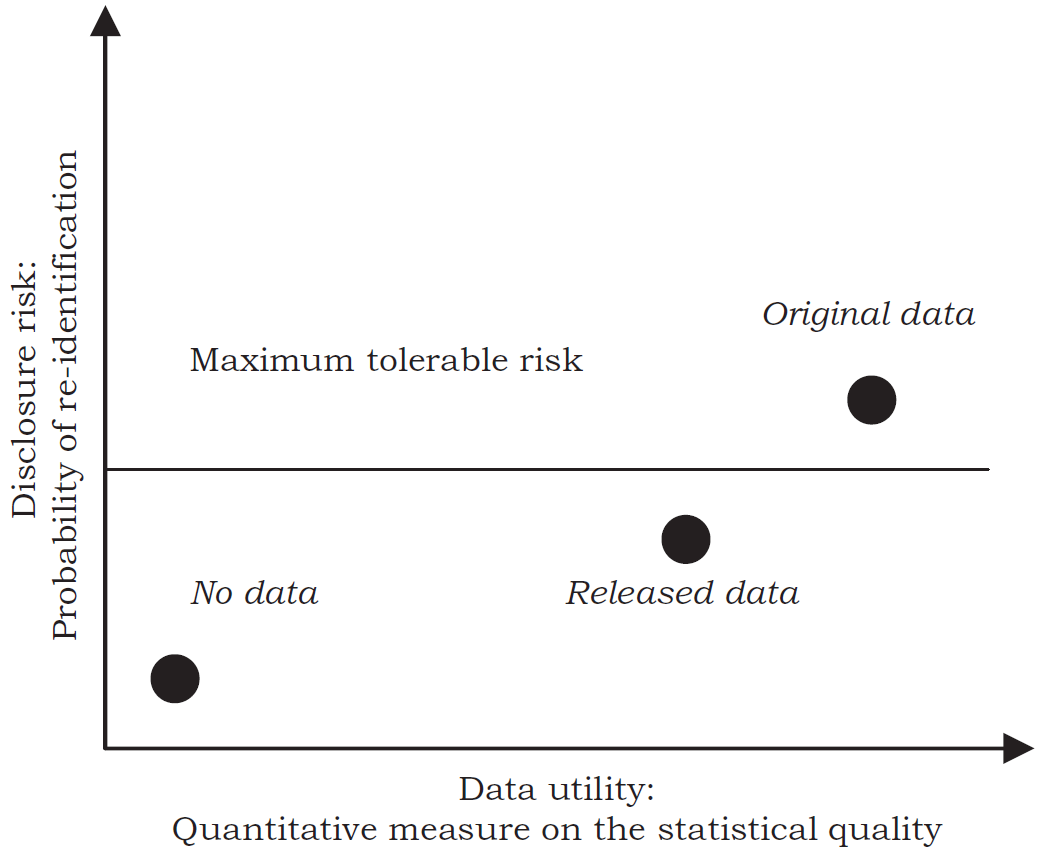
\includegraphics[width=0.5\textwidth,height=\textheight]{gallery/R-U confidentiality map.png}

}

\caption{R-U confidentiality map (Duncan et al.,2001)}

\end{figure}%
\end{frame}

\begin{frame}{k-anonymity}
\phantomsection\label{k-anonymity}
A data set is said to satisfy k-anonymity for k \textgreater{} 1 if, for
each combination of values of quasi-identifiers (e.g.~name, address,
age, gender, etc.), at least k records exist in the data set sharing
that combination.

Ensures that each record is indistinguishable from at least k-1 other
records with respect to the quasi-identifiers.

More robust aproaches:

\begin{itemize}
\item
  \textbf{l-Diversity} Extends k-anonymity by ensuring that the
  sensitive attribute has at least l well-represented values
\item
  \textbf{t-Closeness} Ensures that the distribution of the sensitive
  attribute in any equivalence class is close to the distribution in the
  entire dataset
\end{itemize}
\end{frame}

\begin{frame}{Disclosure risk}
\phantomsection\label{disclosure-risk}
A unit is at risk of disclosure when it cannot be confused with several
other units

\begin{itemize}
\item
  \color{red}{XXX}
\end{itemize}
\end{frame}

\begin{frame}{Re-identification risk}
\phantomsection\label{re-identification-risk}
\begin{itemize}
\item
  \color{red}{attacker scenarios and risk measures in more detail using examples}
\end{itemize}
\end{frame}

\begin{frame}{Variables}
\phantomsection\label{variables}
\begin{enumerate}
\item
  \textbf{\emph{Identifiers}} - variables that can directly identify an
  individual
\item
  \textbf{\emph{Quasi-identifiers}} or \textbf{key variables} - these
  variables don't identify individuals on their own but can do so when
  combined with other quasi-identifiers
\item
  \textbf{Confidential outcome variables} - variables that contain
  sensitive information that should be protected
\item
  \textbf{Non-confidential outcome variables} - these are variables that
  are not sensitive and don't risk the privacy of individuals if
  disclosed
\end{enumerate}
\end{frame}

\begin{frame}{Disclosure control methods}
\phantomsection\label{disclosure-control-methods}
\begin{enumerate}
\tightlist
\item
  \textbf{Masking original data}

  \begin{enumerate}
  [i.]
  \tightlist
  \item
    \textbf{Non-perturbative masking} - Methods that alter data to hide
    identities without changing its actual values
  \item
    \textbf{Perturbative masking} - Methods that add noise or alter data
    values to prevent identification
  \end{enumerate}
\item
  \textbf{Generating synthetic data}

  \begin{enumerate}
  [i.]
  \tightlist
  \item
    \textbf{Parametric methods} - Techniques that use statistical models
    based on the data's distribution to generate synthetic data.
  \item
    \textbf{Non-parametric methods} Techniques that do not assume an
    underlying distribution, using methods like bootstrapping to
    generate synthetic data.
  \item
    \textbf{Generative Adversarial Networks (GANs)} Advanced machine
    learning models that generate highly realistic synthetic data by
    training two neural networks in tandem.
  \end{enumerate}
\end{enumerate}
\end{frame}

\begin{frame}{Packages for SDC - Microdata (Unit-level data)}
\phantomsection\label{packages-for-sdc---microdata-unit-level-data}
\href{https://cran.r-project.org/web/packages/sdcMicro/index.html}{\color{blue}\underline{\textbf{sdcMicro}}}
can be used to anonymize data, i.e.~to create anonymized files for
public and scientific use. It implements a wide range of methods for
anonymizing categorical and continuous (key) variables. The package also
contains a graphical user interface, which is available by calling the
function sdcGUI.

\href{https://cran.r-project.org/web/packages/simPop/index.html}{\color{blue}\underline{\textbf{simPop}}}
using linear and robust regression methods, random forests (and many
more methods) to simulate synthetic data from given complex data. It is
also suitable to produce synthetic data when the data have hierarchical
and cluster information (such as persons in households) as well as when
the data had been collected with a complex sampling design. It makes use
of parallel computing internally.

\href{https://cran.r-project.org/web/packages/synthpop/index.html}{\color{blue}\underline{\textbf{synthpop}}}
using regression tree methods to simulate synthetic data from given
data. It~is suitable to produce synthetic data when the data have no
hierarchical and cluster information (such as households) as well as
when the data does not collected with a~complex sampling design.
\end{frame}

\begin{frame}{Packages for SDC - Tabular data (Aggregated data)}
\phantomsection\label{packages-for-sdc---tabular-data-aggregated-data}
\href{https://cran.r-project.org/web/packages/sdcTable/index.html}{\color{blue}\underline{\textbf{sdcTable}}}
can be used to provide confidential (hierarchical) tabular data. It
includes the HITAS and the HYPERCUBE technique and uses linear
programming packages (Rglpk and lpSolveAPI) for solving (a large amount
of) linear programs.

\href{https://cran.r-project.org/web/packages/sdcSpatial/index.html}{\color{blue}\underline{\textbf{sdcSpatial}}}
can be used to smooth or/and suppress raster cells in a map. This is
useful when plotting raster-based counts on a map. sdcHierarchies
provides methods to generate, modify, import and convert nested
hierarchies that are often used when defining inputs for statistical
disclosure control methods.

\href{https://cran.r-project.org/web/packages/SmallCountRounding/index.html}{\color{blue}\underline{\textbf{SmallCountRounding}}}
can be used to protect frequency tables by rounding necessary inner
cells so that cross-classifications to be published are safe.

\href{https://cran.r-project.org/web/packages/GaussSuppression/index.html}{\color{blue}\underline{\textbf{GaussSuppression}}}
can be used to protect tables by suppression using the Gaussian
elimination secondary suppression algorithm.
\end{frame}

\begin{frame}{Non-perturbation methods}
\phantomsection\label{non-perturbation-methods}
Non-perturbative masking does not rely on distortion of the original
data but on partial suppressions or reductions of detail.

\begin{longtable}[]{@{}lcc@{}}
\caption{Non-perturbative methods vs.~data types.}\tabularnewline
\toprule\noalign{}
Method & Continuous data & Categorical data \\
\midrule\noalign{}
\endfirsthead
\toprule\noalign{}
Method & Continuous data & Categorical data \\
\midrule\noalign{}
\endhead
Sampling & & X \\
Global recoding & X & X \\
Top and bottom coding & X & X \\
Local suppression & & X \\
\bottomrule\noalign{}
\end{longtable}
\end{frame}

\begin{frame}{sdcMicro}
\phantomsection\label{sdcmicro}
\begin{itemize}
\item
  sdcMicro is an R package for statistical disclosure control.
\item
  \url{https://cran.r-project.org/web/packages/sdcMicro/index.html}
\item
  \url{https://github.com/sdcTools/sdcMicro}
\end{itemize}
\end{frame}

\begin{frame}{sdcMicro}
\phantomsection\label{sdcmicro-1}
\begin{figure}[H]

{\centering 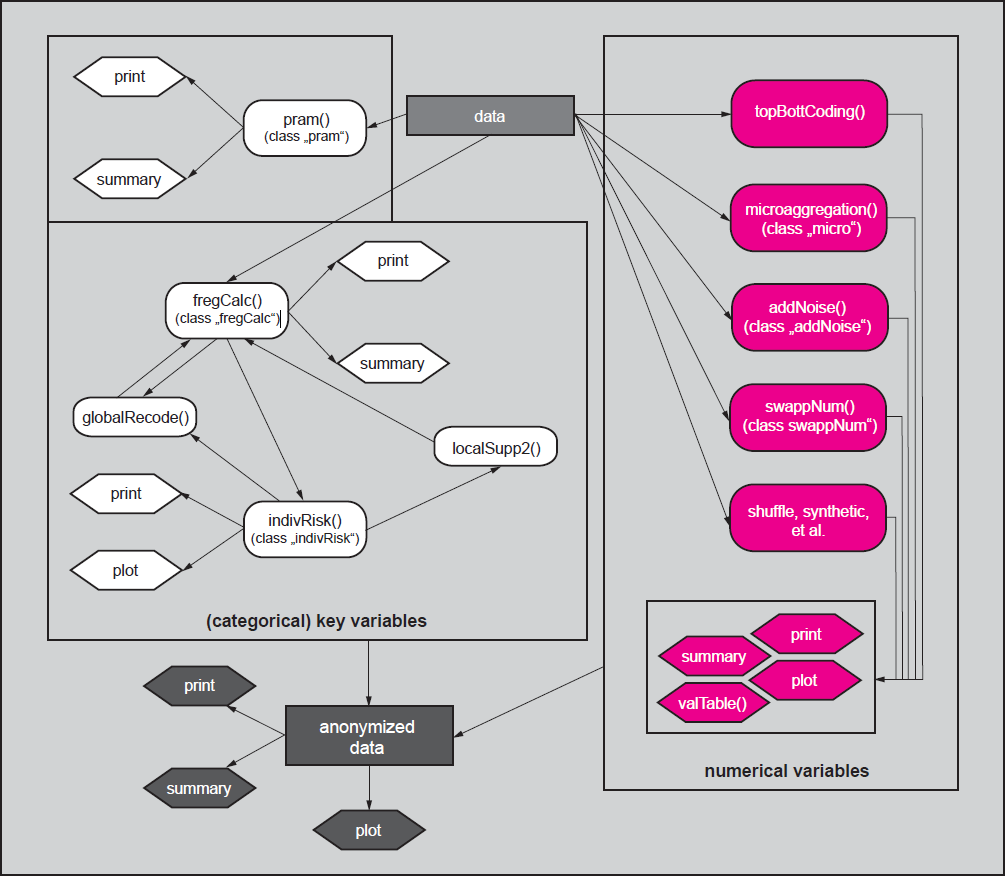
\includegraphics[width=0.55\textwidth,height=\textheight]{gallery/sdcMicro.png}

}

\caption{Certain procedures in package \emph{sdcMicro} and their
relationship}

\end{figure}%
\end{frame}

\begin{frame}{Perturbation methods}
\phantomsection\label{perturbation-methods}
\begin{itemize}
\item
  \begin{itemize}
  \item
    \color{red}{sdcMicro}
  \end{itemize}
\end{itemize}
\end{frame}

\begin{frame}{Synthetic methods}
\phantomsection\label{synthetic-methods}
\begin{itemize}
\item
  \color{red}{Introduction to synthetic data}
\item
  \Huge \color{red}{for Jiri/Oscar}
\end{itemize}
\end{frame}

\begin{frame}{Synthetic methods: synthpop}
\phantomsection\label{synthetic-methods-synthpop}
\begin{itemize}
\item
  \color{red}{Generating synthetic data with synthpop}
\item
  \Huge \color{red}{for Jiri/Oscar}
\end{itemize}
\end{frame}

\begin{frame}{Synthetic methods: synthpop}
\phantomsection\label{synthetic-methods-synthpop-1}
Nowok B, Raab GM, Dibben C (2016). synthpop: Bespoke Creation of
Synthetic Data in R. Journal of Statistical Software, 74(11), 1-26.
doi:10.18637/jss.v074.i11. URL
\href{https://www.jstatsoft.org/article/view/v074i11}{\color{blue}\underline{\textbf{https://www.jstatsoft.org/article/view/v074i11}}}
\end{frame}

\begin{frame}{Synthetic methods: simPop}
\phantomsection\label{synthetic-methods-simpop}
\begin{itemize}
\item
  \color{red}{Generating synthetic data with simPop}
\item
  \Huge \color{red}{for Jiri/Oscar}
\end{itemize}
\end{frame}

\begin{frame}{Synthetic methods: simPop}
\phantomsection\label{synthetic-methods-simpop-1}
Meindl B, Templ M, Alfons A, Kowarik A (2016). simPop: Simulation of
Synthetic Popula- tions for Survey Data Considering Auxiliary
Information. R package version 0.3.0, URL
\href{https://CRAN.R-project.org/package=simPop}{\color{blue}\underline{\textbf{https://CRAN.R-project.org/package=simPop}}}

Parametric and non-parametric methods.
\end{frame}

\begin{frame}{Synthetic methods: GANS}
\phantomsection\label{synthetic-methods-gans}
\begin{itemize}
\item
  \color{red}{Generating synthetic data with GANs}
\item
  \Huge \color{red}{for Marco}
\end{itemize}
\end{frame}

\begin{frame}{}
\phantomsection\label{section}
\centering

\Huge Thank you for your attention\\


\includegraphics[width=0.8\textwidth,height=\textheight]{style/SwissAnon.png}

\large Swiss Data Anonymization Competence Center

\href{https://swissanon.ch}{\color{blue}\underline{https://swissanon.ch}}
\end{frame}



\end{document}
